\documentclass{beamer}
\usepackage{graphicx}

\title{Generative modelling of RNA 3D Modules}
\author{Carlos G. Oliver}
\date{\today}
\graphicspath{{Figures/}}

\begin{document}

\frame{\titlepage}


\frame
{
	\frametitle{Background}
	
	\begin{figure}
		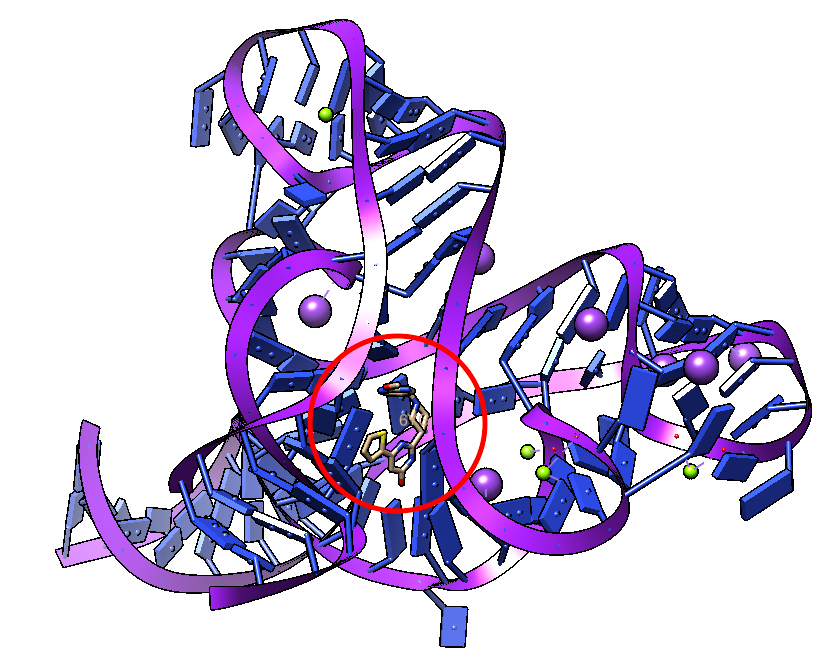
\includegraphics[width=0.7\textwidth]{riboswitch.png}
	\end{figure}
	

}


\frame
{
  \frametitle{Problem}
  
  Automated pipeline for sequence-based RNA-ligand interactions.
  
  \begin{figure}
  	\centering
	 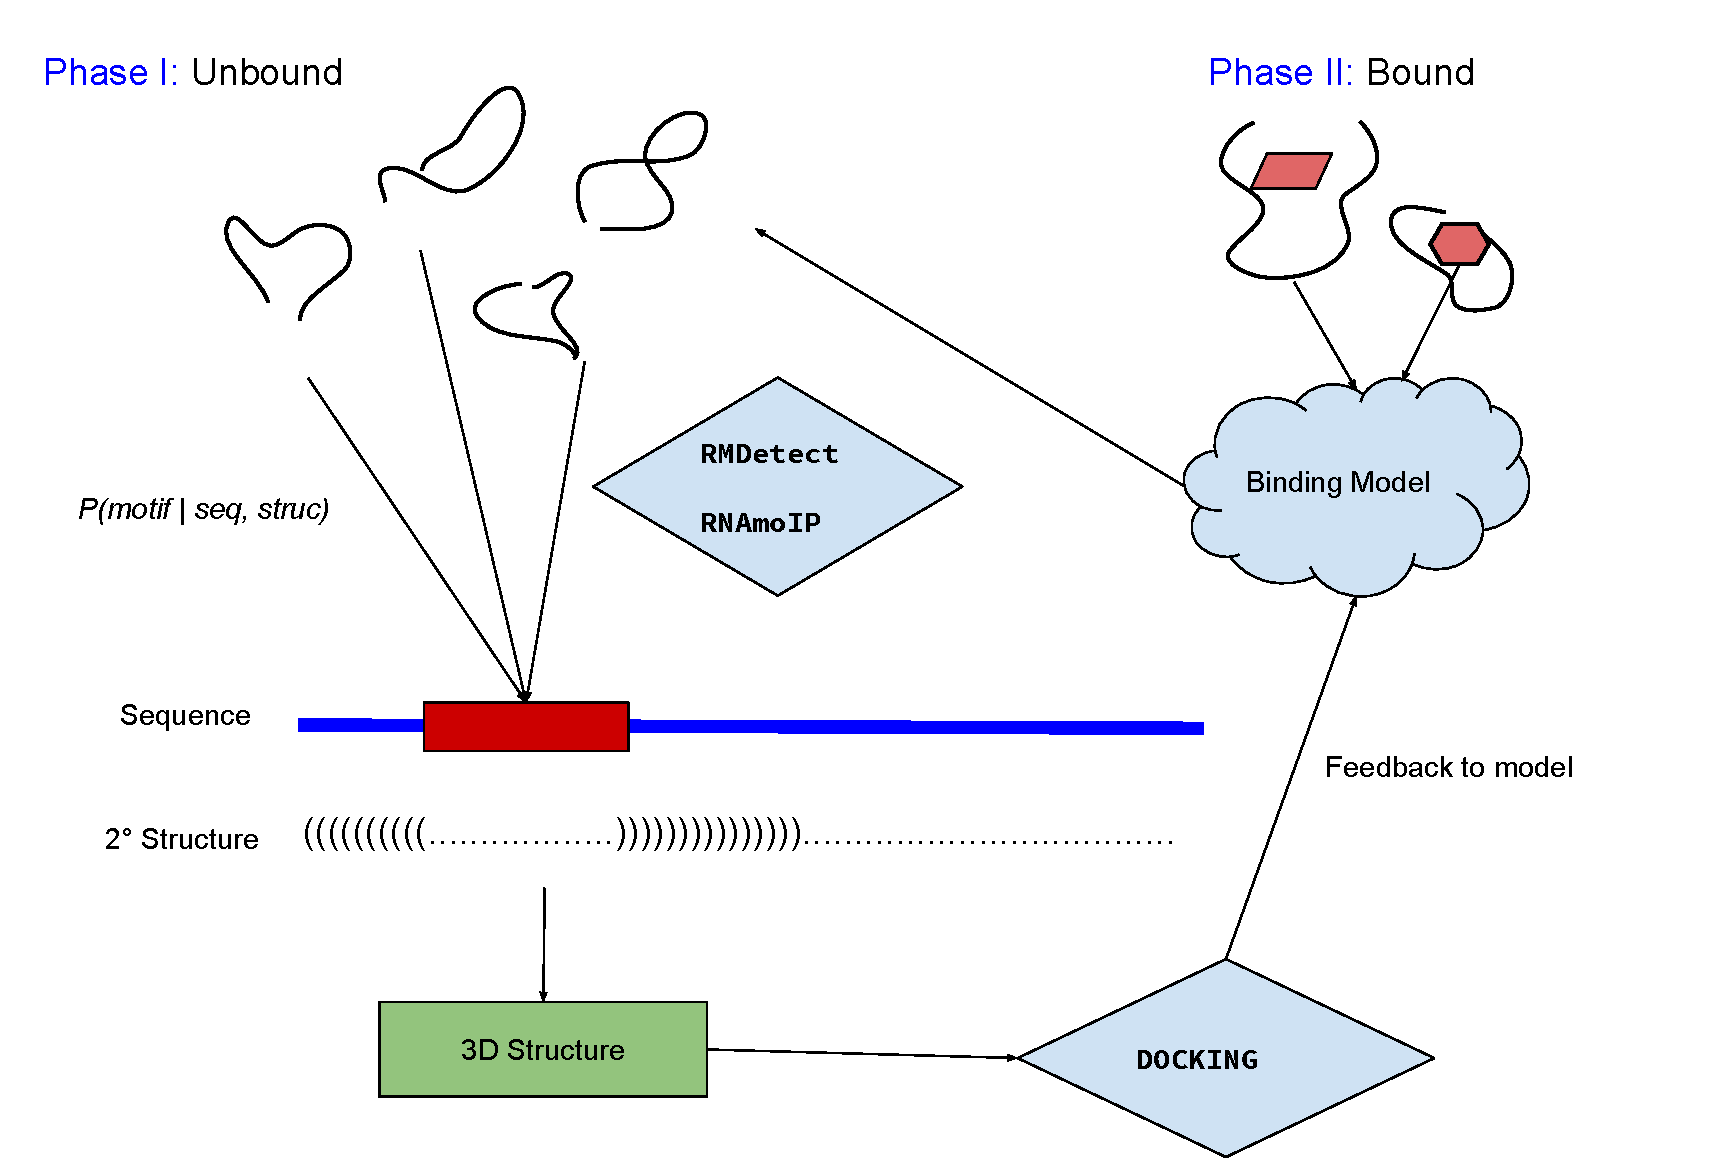
\includegraphics[width=0.8\textwidth]{RiboCop_Diagram.pdf}
  \end{figure}

  }
  
  \frame
  {
  	\frametitle{Data}
	
	Full atomic structures of 4,600 non-redundant RNA-3D modules.
	
	\begin{figure}
		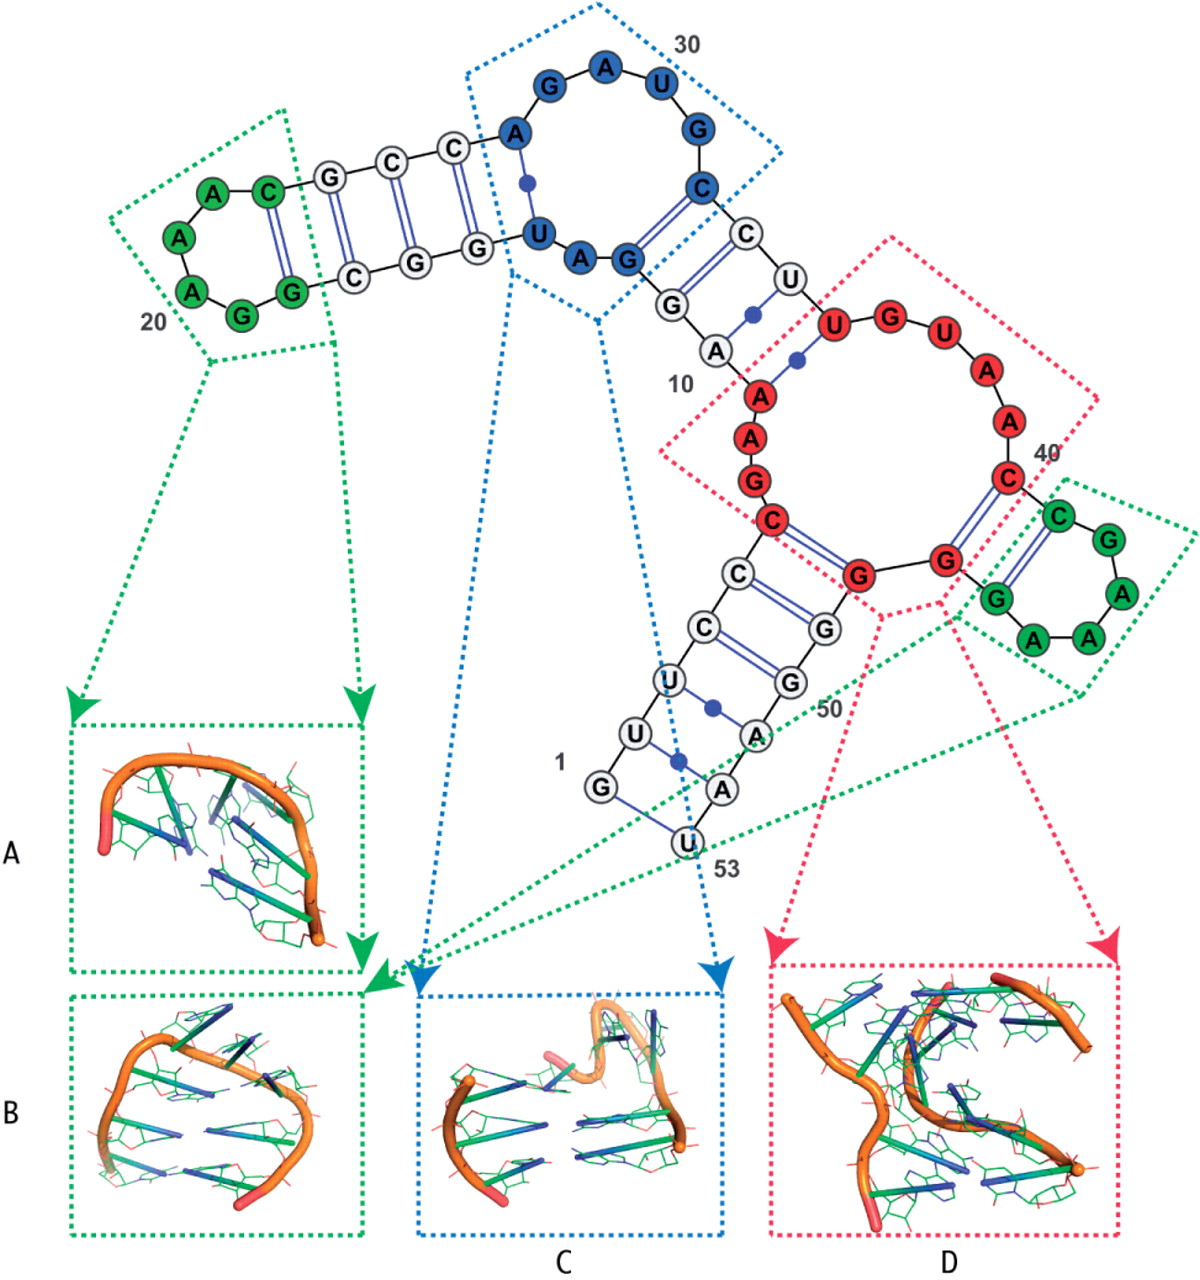
\includegraphics[width=0.6\textwidth]{motifs.jpeg}
	\end{figure}
  
  }
\end{document}
